\documentclass[tikz,border=10pt]{standalone}
\begin{document}
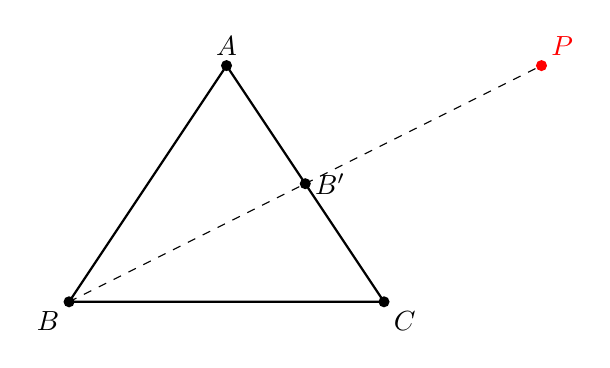
\begin{tikzpicture}

    % Define the points
    \coordinate (A) at (0, 3);
    \coordinate (B) at (-2, 0);
    \coordinate (C) at (2, 0);
    \coordinate (P) at (4, 3);
    \coordinate (Bdash) at (1,1.5);

    % Draw the triangle ABC
    \draw[thick] (A) -- (B) -- (C) -- cycle;

    % Draw the point P
    \fill[red] (P) circle (2pt) node[above right] {$P$};

    \draw[dashed] (B) -- (Bdash);
    
    \draw[dashed] (Bdash) -- (P);
    

    % Label the vertices
    \fill[black] (A) circle (2pt) node[above] {$A$};
    \fill[black] (B) circle (2pt) node[below left] {$B$};
    \fill[black] (C) circle (2pt) node[below right] {$C$};
    \fill[black] (Bdash) circle (2pt) node[ right] {$B'$};

\end{tikzpicture}
\end{document}